\tikzset{
	treenode/.style={align=center,inner sep=0pt},
	% Black nodes
	node_black/.style={treenode,circle,white,font=\bfseries, draw=black, fill=black, text width=0.8cm},
	% Red nodes
	node_red/.style={treenode,circle,red,draw=red,very thick,text width=0.8cm},
	% Nil nodes
	node_nil/.style={treenode,rectangle,fill=black,minimum width=0.3cm,minimum height=0.3cm}
}

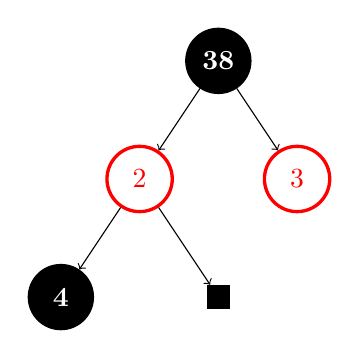
\begin{tikzpicture}[->,level/.style={sibling distance=2cm, level distance=1.5cm}]
	\node[node_black]{38}	
		child{node[node_red]{2}
			child{node[node_black]{4}}
			child{node[node_nil]{}}
		 	}
		child{node[node_red]{3}}	
	
	;
\end{tikzpicture}

%%--------------------------------------
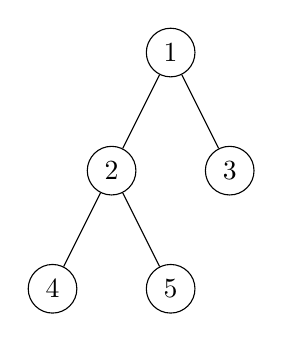
\begin{tikzpicture}[every node/.style={circle, draw=black}]

\node{1}
	child{node{2}
		child{node{4}}
		child{node{5}}
		 }
	child{node{3}};
\end{tikzpicture}

%%--------------------------------------




%%--------------------------------------